\subsubsection{Removing hidden categories}
\label{sec:removing_hidden_categories}
Wikipedia's category structure contains lots of hidden categories which are not displayed as categories at the bottom of an article page for the general users, even if the article is placed under the category. Examples of some hidden categories are \emph{All articles with dead external links}, \emph{Wikipedia Articles needing rewrite} and \emph{Wikipedia articles in need of updating from September 2014}. Hidden categories are useful for editing articles or maintaining a trustworthy and well-structured encyclopedia. These categories provide an easy way to mark all  categories with something in common, for instance mark all categories with references that needs to be checked. 

Hidden categories are concerned with maintenance and administration, hence not relevant for normal users, or for our project for 2 reasons: 
\begin{enumerate}
\item Hidden categories do not provide relevant information in full article paths.
\item Hidden categories add complexity to our structure.
\end{enumerate}
Hence, it is desirable to remove all links to hidden categories, which means that we need the titles of all hidden categories.  On Wikipedia's information page about the category \emph{Hidden Categories}\cite{wiki:hiddencat} 15 385 subcategories are listed as immediate subcategories, which means that these are also hidden categories. Many of these categories have links to their own hidden subcategories. We did two attempts for finding all hidden categories. The first attempt was to look through all the links from the category \emph{Hidden Categories}, where 15 006 subcategories where found and marked as not relevant. This did not give the expected number, so the second attempt was made by looking at the file \enwikipageprops. All ids marked with \emph{hiddencat} (see figure \ref{fig:pageprops}) were collected and their corresponding category title found in \enwikipage. This approach led to 15 513 categories. To make sure that all hidden categories where found, a test was made to see if all categories from the first attempt was found in the list created from the second attempt. The results showed that all categories found in the first attempt was also found in the second attempt, and the list of all 15 513 category titles whose links should be disregarded from the paths in the final results. 

\begin{figure}[h]
\centering
\begin{lstlisting}
(747593,'hiddencat','',NULL)
\end{lstlisting}
\caption[Insert statement for hidden category]{Excerpt from the file \texttt{enwiki-latest-page\_props.sql.gz} where we can see that hidden categories are marked with \emph{hiddencat}}
\label{fig:pageprops}
\end{figure}

The hidden categories should be removed from both links between categories and articles, and between categories. The first case is easy since the links can just be removed from the results. Removing hidden categories between categories has to be done carefully to make sure that information is not lost. Hidden categories might be subcategories of visible categories or have visible categorise as their own subcategories. Figure \ref{fig:stevie_wonder_hidden} is an example of a path to the article about \emph{Stevie Wonder} which includes a hidden category. 


%An example of this can be seen in figure \ref{fig:stevie_wonder_hidden}, where the double rounded rectangle is a hidden category, the rounded rectangle is a normal (visible) category and the rectangle is the article about \emph{Stevie Wonder}.


%Hidden categories can not be disregard
%19103360 article links, 391482 category links skipped

%An example of such a structure can be found from the categories leading to the article about the singer Stevie Wonder. 

\begin{figure}[h]
\centering
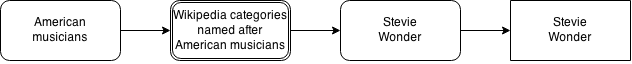
\includegraphics[width=\textwidth]{Chapters/Implementation/HiddenCategories/Stevie_wonder_hidden}
\caption[Example path with hidden category]{An excerpt of one path leading to the article about to Stevie Wonder, where the path contains a hidden category. }
\label{fig:stevie_wonder_hidden}
\end{figure}

The desirable visible paths for all articles are paths without hidden categories. Thus, the hidden categories should be removed from the structure without loosing any of the subcategories which might contain relevant information or  important links. Example of a how a path can be transformed is figure \ref{fig:stevie_wonder} which is the excerpt from the path in figure \ref{fig:stevie_wonder_hidden} without the hidden categories. 

\begin{figure}[h]
\centering
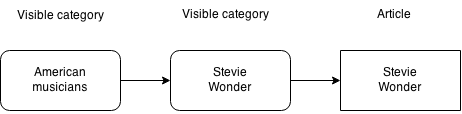
\includegraphics[width=.7\textwidth]{Chapters/Implementation/HiddenCategories/Stevie_wonder}
\caption[Example path without hidden category]{The desirable output of the excerpt of the path leading to the article about Stevie Wonder where the hidden category is removed from the path}
\label{fig:stevie_wonder}
\end{figure}

Table \ref{tab:withouthiddencat} shows how number of links between categories and articles are reduced when hidden categories are disregarded. Number of links between categories has increased even though total number of categories are reduced from 519 822 to 504 309.

%The main reason to reduce number of links is to reduce the complexity 

\begin{table}[h]
\centering
\renewcommand{\arraystretch}{1.25}
\begin{tabular}{l|c|c}
\textbf{Links between...} & \textbf{W/ Hidden Categories} & \textbf{W/o Hidden Categories}  \\ \hline
 \textbf{subcategories} & 3 358 007  & 3 467 360\\
 \textbf{articles and categories} & 71 487 647  & 52 611 629 
\end{tabular}
\\[10pt]
\caption[Number of links without hidden categories]{Number of links removed when all hidden categories are excluded. }
\label{tab:withouthiddencat}
\end{table}




\begin{comment}

504309 + 15513

Number of category links (w hiddencats): 3 358 007
Number of category links (w/o hiddencats): 

Number of categories before hidden cats: 1 206 719
Number of categories (after hidden cats): 1199730

Number of hidden categories: 1964

3 358 008
3 467 360

Difference in number of categories: 1 654 758  & 1 311 275

[INFO] Diambiguation links found: 285624
[INFO] Writing category links to file
[INFO] --- 1194.24166107 seconds (19.9040276845 min, 54.2416610718 min) ---
[INFO] 18898753 article links, 0 category links skipped

1648873 sub categories written to S.txt.gz
2948243 page categories written to P.txt.gz
22735 number links between categories or cat-articles found

artskip: 18898753
filecnt : 5262146
insertioncnt : 88172914 

Lines read 88172914

 & 5 262 146 & 2948243
\end{comment}